\section{Large language model adoption in agent-based modeling}

\subsection{What changed, and what did not}

For this review, 2018–2022 is treated as the pre-LLM comparison period and 2023–2025 as the post-release observation period, with late 2022 as the historical boundary associated with ChatGPT’s public release. This is a periodization device, not a causal design. A before–after comparison can identify temporal reorientation, but it cannot prove that LLMs caused changes in topic choice or collaboration.

The pre/post comparison shows continuity among the highest-ranked subthemes alongside changes elsewhere in the distribution. Epidemiological modeling and opinion dynamics remain first and second in both periods. Social network analysis rises from fourth to third, social influence from fifth to fourth, urban planning from eleventh to sixth, and ABM as a named method from twelfth to eighth; information diffusion also enters the post-release top twenty. In contrast, population dynamics moves from third to fifth, disease-spread modeling from sixth to eighteenth, cost-effectiveness from seventh to twelfth, and wildlife conservation from tenth to twentieth. These are relative rankings among leading subthemes, not measures of absolute publication volume. The pattern is consistent with greater visibility for networked interaction, influence, and information-related questions, but this descriptive comparison cannot attribute the changes to LLMs or to any single historical event.

\begin{figure}[htbp]
\centering
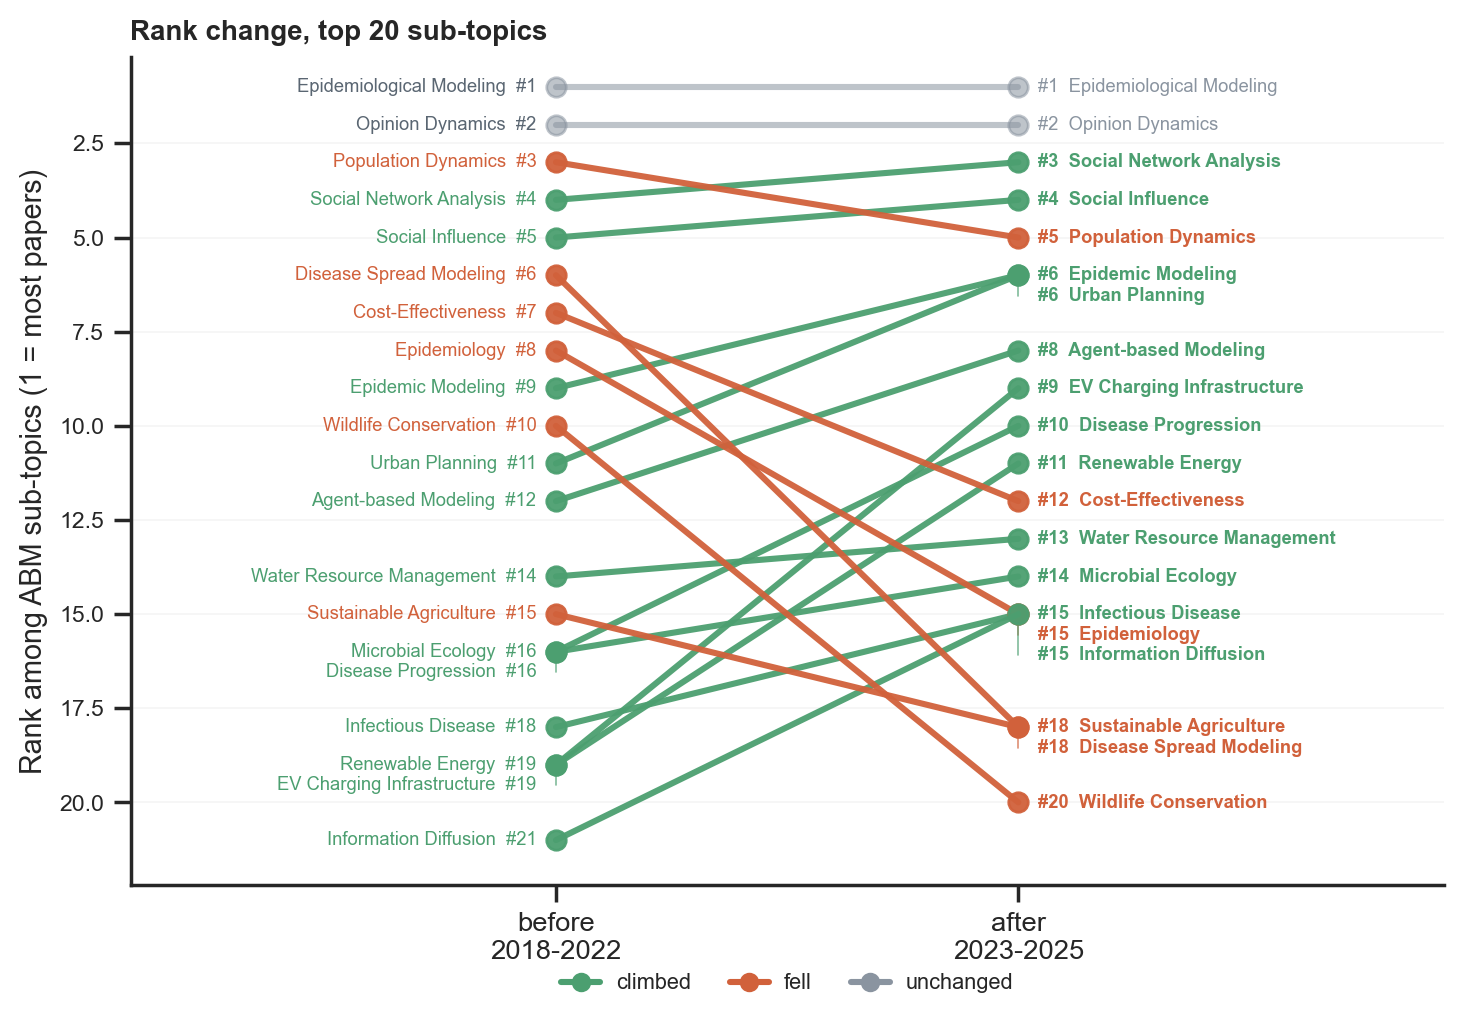
\includegraphics[width=0.96\textwidth,height=0.78\textheight,keepaspectratio]{figures/figure_10.png}
\setcounter{figure}{6}
\caption{Rank changes among leading subthemes before and after the public emergence of ChatGPT.}
\label{fig:figure7}
\end{figure}

\begin{table}[htbp]
\centering
\scriptsize
\setlength{\tabcolsep}{3pt}
\renewcommand{\arraystretch}{1.18}
\setcounter{table}{1}
\caption{}
\label{tab:table2}
\begin{tabularx}{\linewidth}{>{\raggedright\arraybackslash}p{0.15\linewidth} *{4}{>{\raggedright\arraybackslash}X}}
\toprule
\textbf{Dimension} & \textbf{Before LLM diffusion (2018–2022)} & \textbf{Early post-LLM period (2023–2025)} & \textbf{Evidence in corpus} \\
\midrule
Research focus & Population, disease, ecology, and established simulation domains & Social networks, influence, information diffusion, and socio-technical systems & Subtheme rank shifts \\
LLM adoption & Not a regular modeling component & 1.50\% → 2.75\% → 5.65\% annually & Cochran–Armitage trend p < 0.001 \\
Primary role & Hand-coded rules and conventional computational tools & Behavioral rules/decision mechanisms plus tool support & 59.6\% internal; 40.4\% instrumental \\
Modeled entity profile & Humans and biological entities within established ABM traditions & More software/computational agents among LLM papers & Software agents +11.5 pp; biological entities −12.7 pp \\
Collaboration & Growing team science already underway & LLM papers show lower international collaboration & 20.3\% vs 31.6\%; q = 5.5 × 10−4 \\
\bottomrule
\end{tabularx}
\end{table}

Table 2. A descriptive comparison of ABM before and after the public emergence of LLMs. The comparison is associational, not causal.

\subsection{Diffusion is accelerating but remains at an early stage}

LLM use grew rapidly from a small base. Of the 29,139 papers in the corpus through 2025, 236 (0.81\%) were classified as using an LLM. Annual counts increased from 32 in 2023 to 63 in 2024 and 141 in 2025. Using the annual denominator applied in the corpus trend analysis, the corresponding shares rose from 1.50\% to 2.75\% and 5.65\%, a 2025-to-2023 rate ratio of 3.77. Despite this clear increase, LLM use was not standard practice by 2025: most ABM papers in the observation window were not classified as LLM-enabled. Because the post-release series covers only three years, it should be read as an early-diffusion snapshot, not a settled trajectory.

\begin{figure}[htbp]
\centering
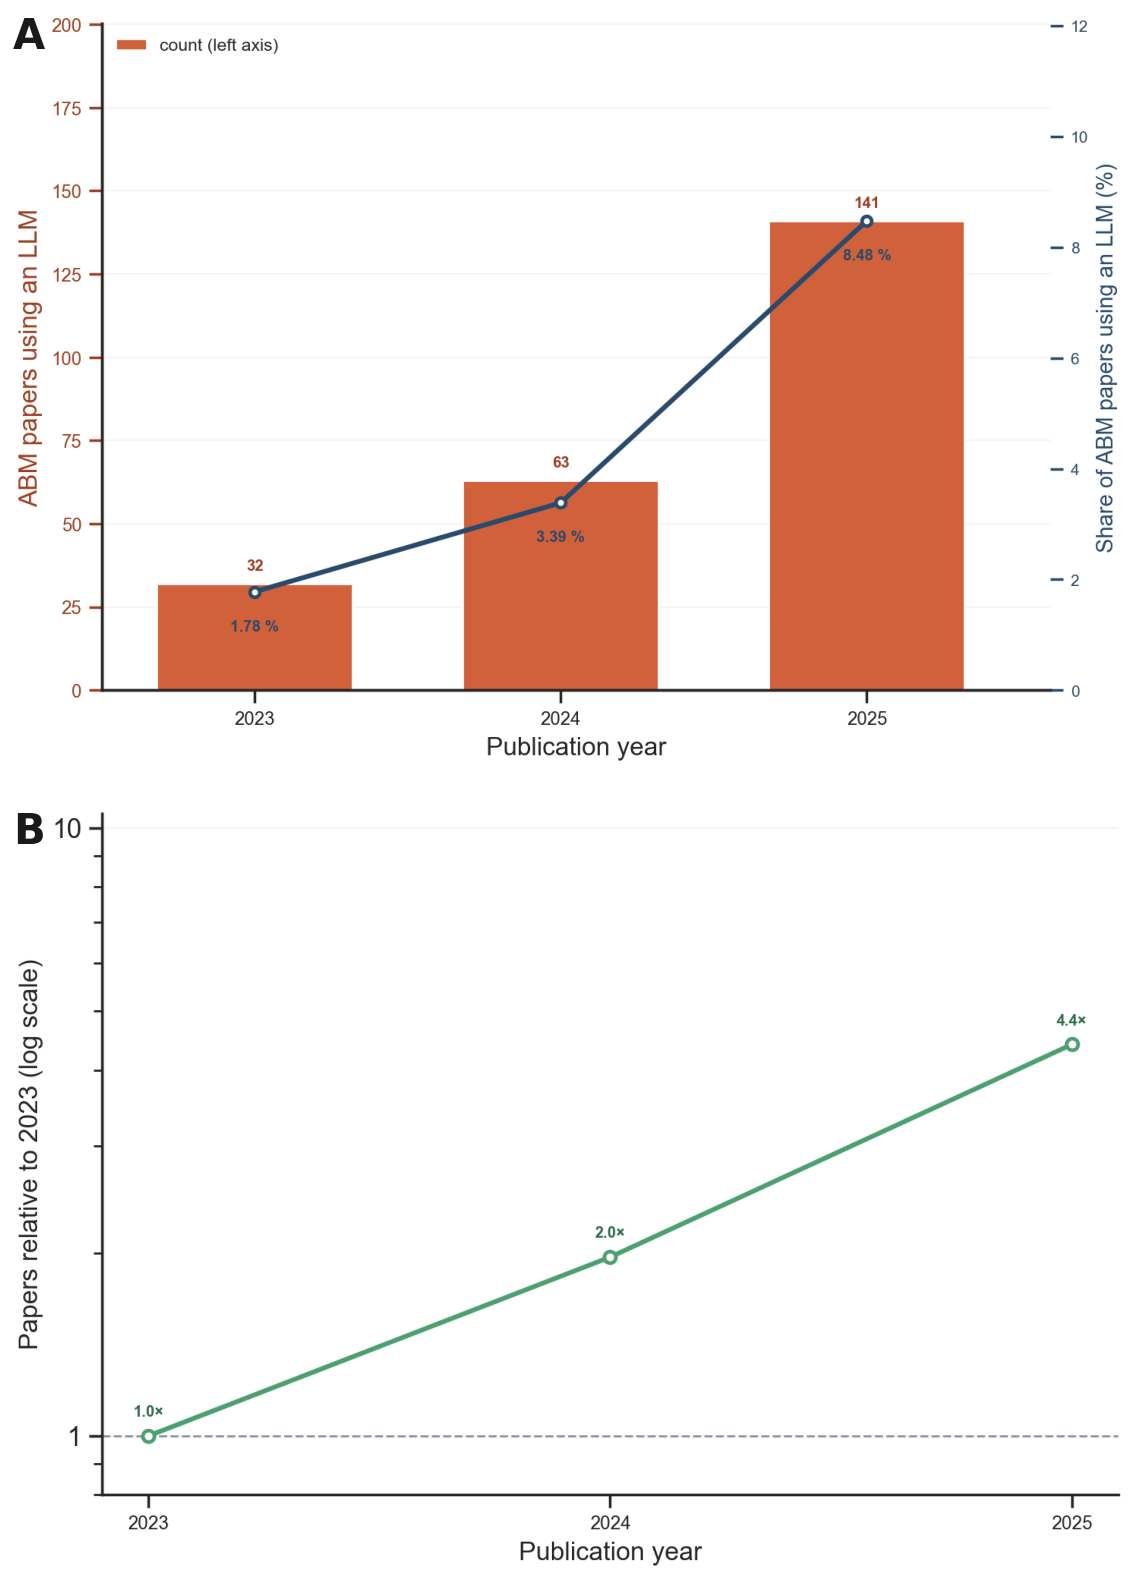
\includegraphics[width=0.96\textwidth,height=0.78\textheight,keepaspectratio]{figures/figure_11.png}
\setcounter{figure}{10}
\caption{LLM adoption over time and index relative to 2023.}
\label{fig:figure11}
\end{figure}

The LLM’s function is as important as its presence. Of 235 papers with a classifiable role, 140 (59.6\%; Wilson 95\% CI 53.2–65.6) used the model in agent behavior or decision-making. The other 95 papers (40.4\%) used LLMs in supporting roles, including code or model implementation, data and parameter generation, evaluation or text analysis, and natural-language interfaces. The corpus thus shows two concurrent patterns: LLMs can form part of the simulated decision mechanism, or support the research workflow around it. These roles should be distinguished because only the former directly changes how simulated agents generate behavior.

\begin{figure}[htbp]
\centering
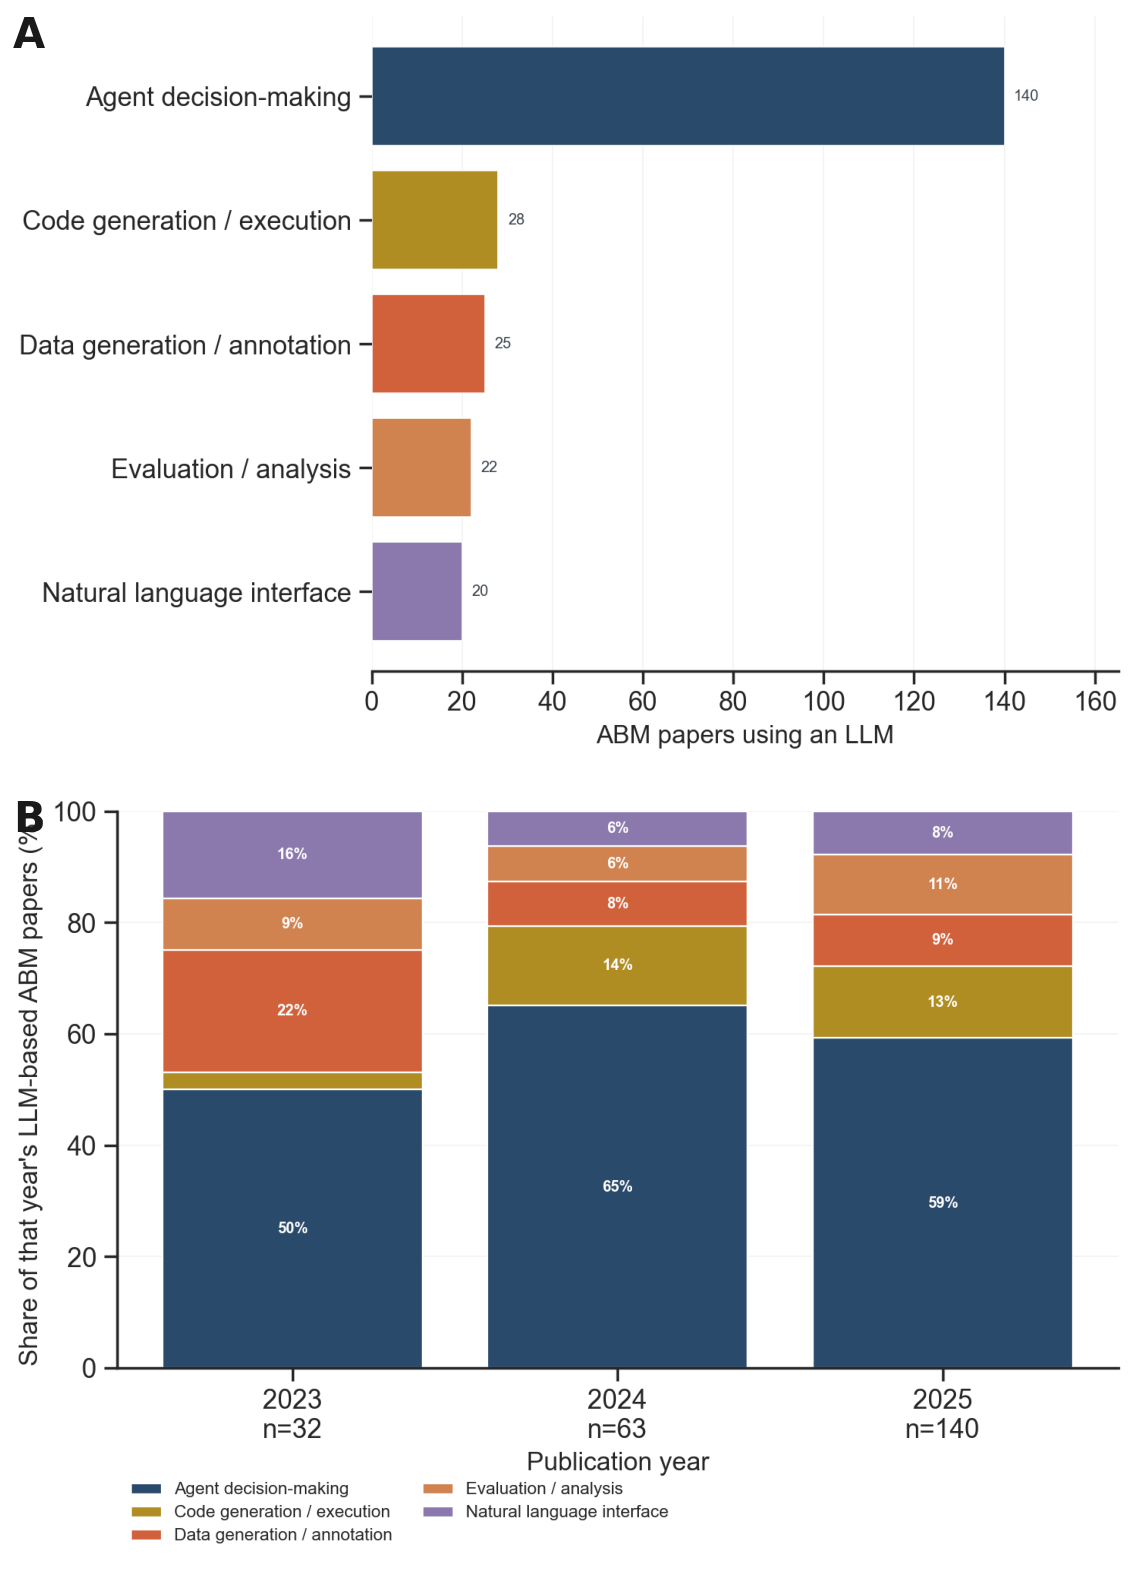
\includegraphics[width=0.96\textwidth,height=0.78\textheight,keepaspectratio]{figures/figure_12.png}
\setcounter{figure}{11}
\caption{Functional roles of LLMs in ABM and their annual composition.}
\label{fig:figure12}
\end{figure}

\begin{figure}[htbp]
\centering
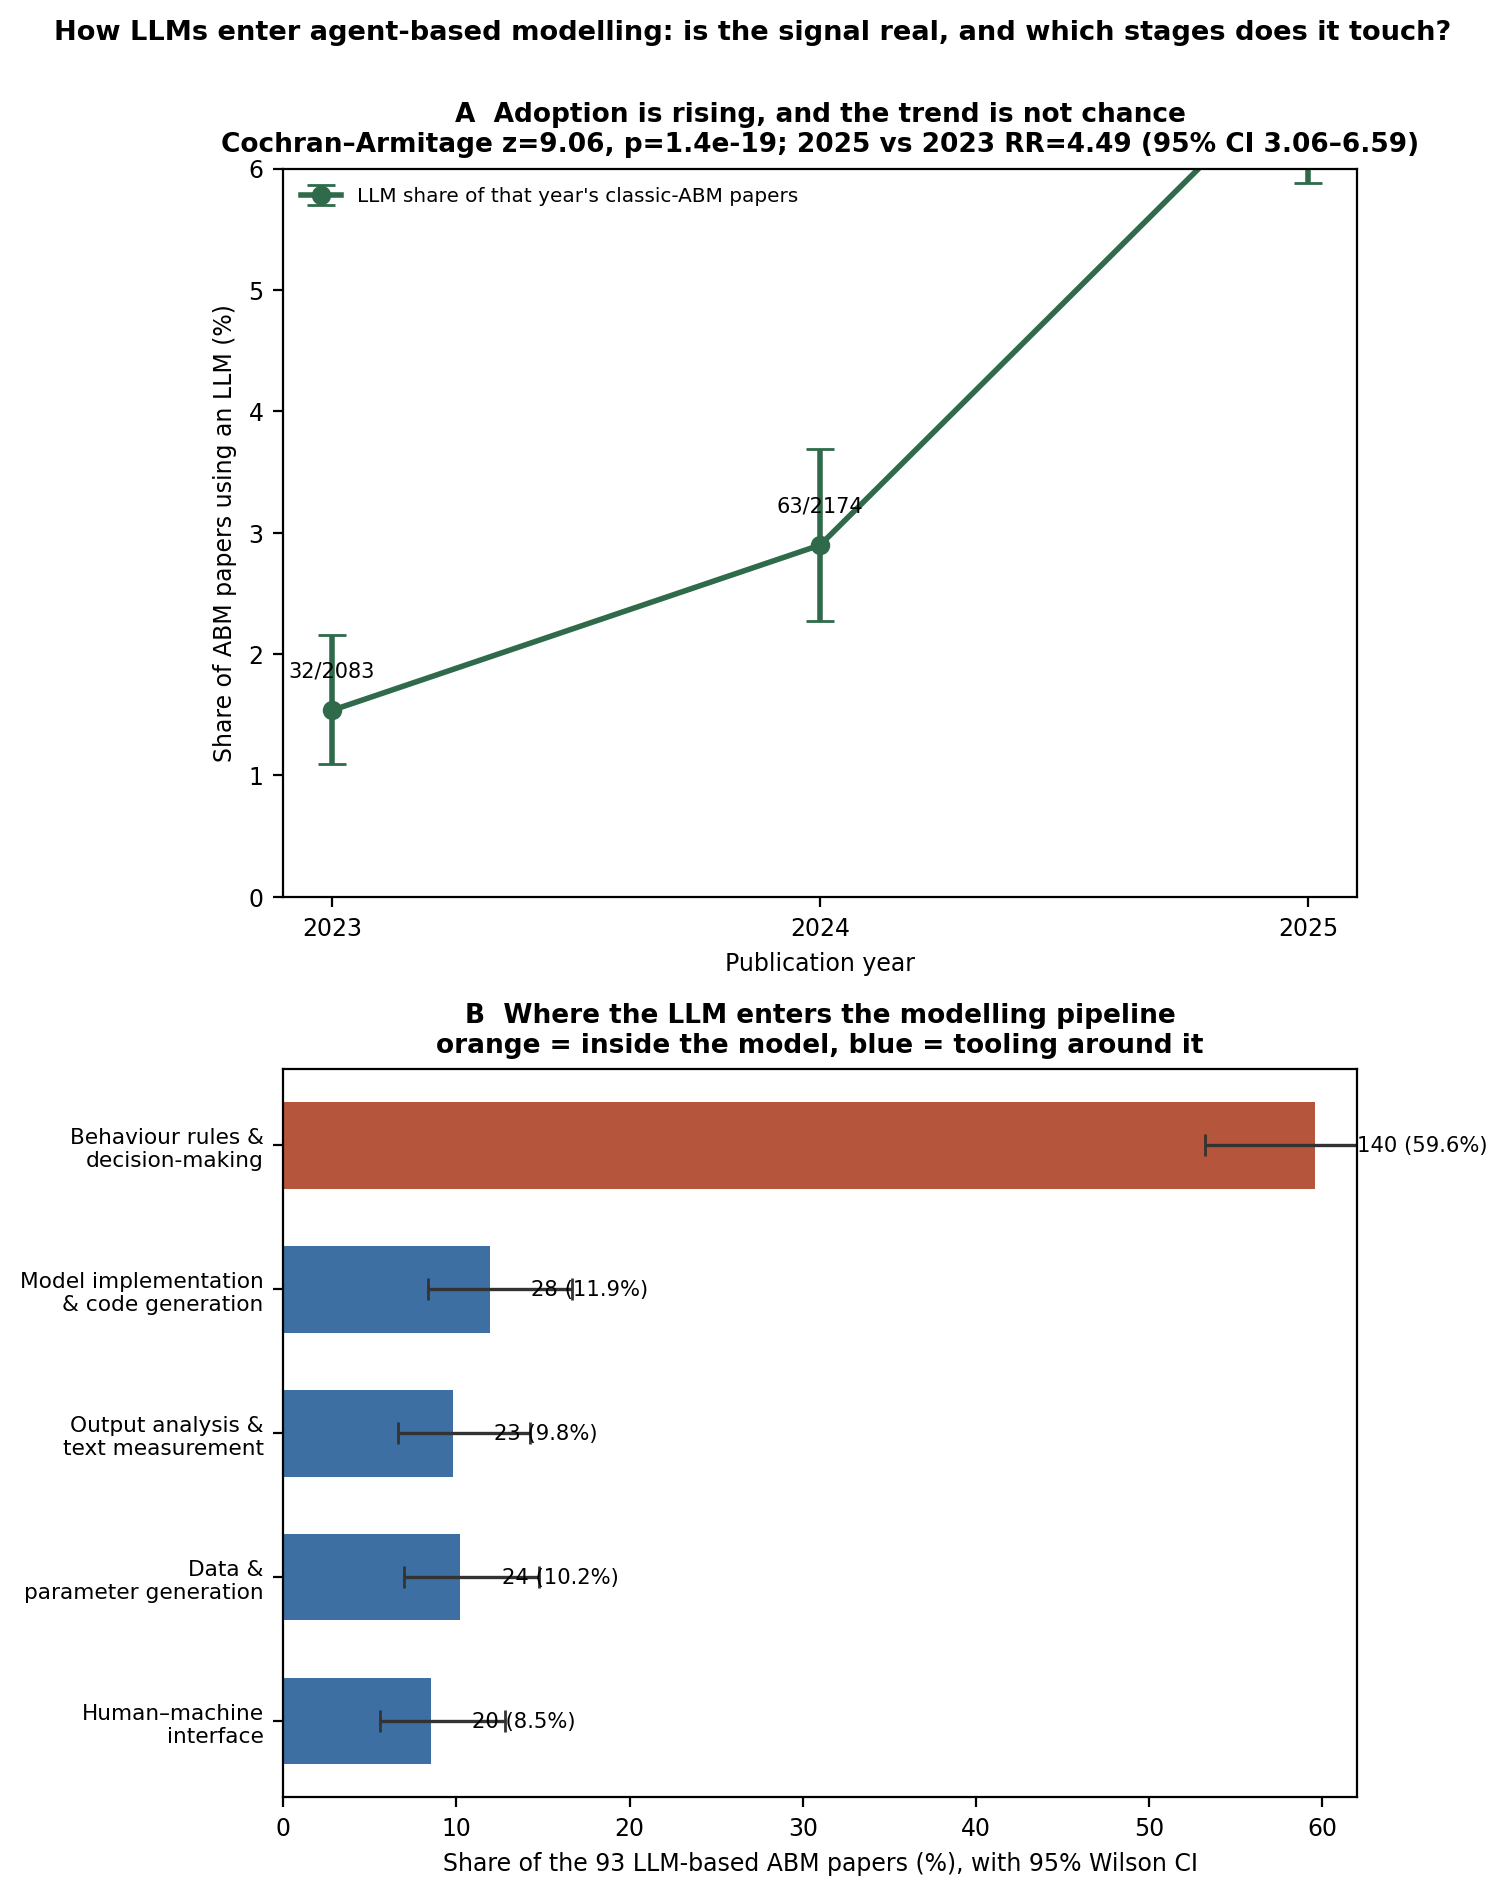
\includegraphics[width=0.96\textwidth,height=0.78\textheight,keepaspectratio]{figures/figure_13.png}
\setcounter{figure}{12}
\caption{Entry points of LLMs into the ABM workflow: adoption tests and modeling-stage location.}
\label{fig:figure13}
\end{figure}

The key transition is the use of LLMs within agents’ decision processes, rather than only as tools for programming, text analysis, or data processing. Conventional ABMs typically specify decision rules directly; LLM-based agents can instead interpret context, retrieve memories, plan, and interact in natural language. Such capabilities may represent flexible, context-dependent behavior that fixed rules are less suited to capture. They do not, on their own, establish that the resulting behavior is valid. \footnote{Park, J. S., O’Brien, J. C., Cai, C. J., Morris, M. R., Liang, P., \& Bernstein, M. S. (2023). Generative agents: Interactive simulacra of human behavior. In Proceedings of the 36th Annual ACM Symposium on User Interface Software and Technology. https://doi.org/10.1145/3586183.3606763} \footnote{Huang, Q., Vora, J., Liang, P., \& Leskovec, J. (2024). Large language models empowered agent-based modeling and simulation: A survey and perspectives. Humanities and Social Sciences Communications, 11, 1259. https://doi.org/10.1057/s41599-024-03611-3; Wang, L., Ma, C., Feng, X., Zhang, Z., Yang, H., Zhang, J., Chen, Z., Tang, J., Chen, X., Lin, Y., Zhao, W. X., Wei, Z., \& Wen, J.-R. (2024). A survey on large language model based autonomous agents. Frontiers of Computer Science, 18(6), 186345. https://doi.org/10.1007/s11704-024-40231-1}

\subsection{Limits of current LLM-enabled ABM and research priorities}

The available evidence supports treating LLM-enabled ABM as an emerging extension of established ABM, not as its replacement. LLM-driven agents still need to represent bounded rationality, adaptation, spatial and network constraints, and institutional rules, and their behavior must be calibrated and validated against empirical evidence. Linguistically coherent, contextually plausible responses are not necessarily stable or behaviorally valid: agents may produce inconsistent choice probabilities, weak demographic differentiation, or implausible policy responses. Outcomes may also vary with model version, prompt, context, stochastic settings, and knowledge-updating procedures. These issues are especially consequential when an LLM serves as the decision engine, because even small changes can alter the simulated behavioral mechanism. \footnote{Ghaffarzadegan, N., Majumdar, A., Williams, R., \& Hosseinichimeh, N. (2024). Generative agent-based modeling: An introduction and tutorial. System Dynamics Review, 40(1), e1761. https://doi.org/10.1002/sdr.1761; Lu, Y., Aleta, A., Du, C., Shi, L., \& Moreno, Y. (2024). LLMs and generative agent-based models for complex systems research. Physics of Life Reviews, 51, 283–293. https://doi.org/10.1016/j.plrev.2024.10.013}

Future research should make uncertainty and validity assessable. Studies should compare LLM-based agents with rule-based and empirically calibrated baselines, then test sensitivity to model version, prompt, random seed, temperature, and information-retrieval strategy. Validation should draw on observed behavior, experiments, or historical cases and should assess both individual decisions and aggregate outcomes. Researchers should also report computational costs, data provenance, privacy safeguards, and how generated outputs were reviewed. Current applications are concentrated in a limited set of areas and cover only the first years of adoption; cross-domain replications and longer time series are therefore needed before general claims about LLMs’ value in ABM are justified.

\emph{Figure 14. Cross-distribution of application domains and LLM roles.}

\subsection{Application domains and simulated agent types}

LLM-enabled ABM is concentrated in a few application areas. Among the 235 papers with classifiable roles in Figure 14, social and opinion dynamics is the largest group (81 papers; 34.5\%), followed by health and epidemiology (58; 24.7\%). Other prominent areas are AI and multi-agent computing (28; 11.9\%), policy and disaster response (25; 10.6\%), sustainability and energy (21; 8.9\%), and transport and urban mobility (18; 7.7\%). Networks and communication and other specialized domains contribute two papers each. This distribution places current work chiefly in social-behavioral and health research, alongside a smaller technical strand in AI and multi-agent systems. Decision-making is the most common LLM function across the major domains; coding, data generation, analysis, and interfaces provide additional routes of use.

The agent types represented in LLM-related studies also differ from those in the broader ABM corpus. Software or computational agents are 11.5 percentage points more prevalent, while biological entities are 12.7 points less prevalent, in the LLM subset. This is consistent with the emergence of software and LLM-based agents as objects of study, but it does not mean that every paper using an LLM simulates an LLM agent. Some use the model to support decisions, data preparation, analysis, or interaction for a different agent population. Separating the LLM’s function from the simulated agent type is therefore essential to interpreting the field’s development.

\subsection{An evaluative framework for LLM-enabled ABM}

The review proposes evaluating LLM-enabled ABM along four dimensions. Behavioral validity asks whether an LLM agent reproduces observed choices, response times, network ties, and switching behavior. Process validity examines whether mechanisms such as memory, planning, social influence, and adaptation remain stable under changes to prompts, seeds, models, or temperature. Macro-level validity tests whether aggregate patterns and policy responses match historical or experimental benchmarks. Governance validity concerns provenance, disclosure of synthetic decisions, protection of sensitive data, and replicability. This framework complements ODD-style documentation with model cards, prompt and version records, stochastic controls, and behavioral benchmarks.